\documentclass{article}
\usepackage[utf8]{inputenc}
\usepackage{graphicx}
\usepackage{float}
\usepackage{amsmath}
\usepackage{listings}
\usepackage{xcolor}
% Definición de colores para el estilo de código
\definecolor{codegreen}{rgb}{0,0.6,0}
\definecolor{codegray}{rgb}{0.5,0.5,0.5}
\definecolor{codepurple}{rgb}{0.58,0,0.82}
\definecolor{backcolour}{rgb}{0.95,0.95,0.92}

\lstset{
    language=Python,
    backgroundcolor=\color{backcolour},   
    commentstyle=\color{codegreen},
    keywordstyle=\color{magenta},
    numberstyle=\tiny\color{codegray},
    stringstyle=\color{codepurple},
    basicstyle=\ttfamily\footnotesize,
    breakatwhitespace=false,         
    breaklines=true,                 
    captionpos=b,                    
    keepspaces=true,                 
    numbers=left,                    
    numbersep=5pt,                  
    showspaces=false,                
    showstringspaces=false,
    showtabs=false,                  
    tabsize=4,
    frame=single
}


\title{Laboratorio 1: El Incidente del Sistema Golgotha}
\author{
    Cristian Quintanilla - 202210117-2 \\
    Jose Alvarado - 202373122-6 \\
    Matias Peñaloza - 202373037-8 \\
    Cristóbal Aguilera - 201741022-1
}
\date{\today}
\begin{document}
\maketitle

\section{Fase 1}
\subsection{Análisis Teórico}
\subsubsection{Generación de Identidad Criptográfica}

La Fase 1 del Protocolo OMEGA establece la raíz de confianza del sistema mediante la vinculación determinista de la identidad del usuario (Nombre y ROL) con sus credenciales criptográficas. A continuación, se detallan los fundamentos técnicos de esta implementación.

\subsubsection{Derivación de la Strong Key mediante PBKDF2}
Para transformar datos de baja entropía en una clave robusta, se utiliza el algoritmo \textit{Password-Based Key Derivation Function 2} (PBKDF2).

\begin{itemize}
    \item \textbf{Función de Estiramiento:} Se emplea HMAC-SHA256 con un factor de iteración de $600,000$. Este alto número de iteraciones aumenta el costo computacional de ataques de fuerza bruta, y es el recomendado por la OWASP para este algoritmo.

\begin{lstlisting}[language=Python, caption=Implementación de derivación de clave con estándar OWASP]
# Derivacion de la Strong Key usando PBKDF2-HMAC-SHA256
strong_key = PBKDF2(
    password=u_rol, 
    salt=salt_utilizado, 
    dkLen=32, 
    count=600000,  # 600k iteraciones segun estandar OWASP 2023
    hmac_hash_module=SHA256
)
\end{lstlisting}
    
    \item \textbf{Uso de SALT:} Se inyecta un \textit{salt} aleatorio de 16 bytes para mitigar ataques de tablas de arcoíris (Rainbow Tables). Esto garantiza que identidades similares produzcan claves únicas.
    La decisión se tomó en base a la recomendación del NIST SP 800-132, que indica una longitud de al menos 128 bits para el SALT.
\end{itemize}

Se evaluó la implementación de Argon2id por su superioridad técnica y resistencia a ataques de GPU (memory-hard). Sin embargo, se optó por PBKDF2 para asegurar la máxima compatibilidad entre los entornos de desarrollo del equipo y la portabilidad del script, compensando su menor resistencia teórica con un alto número de iteraciones ($600,000$).


\subsubsection{Generador Determinista de Números Aleatorios (DRNG)}
Para garantizar la reproducibilidad de las llaves RSA sin depender de la entropía variable del sistema operativo, se implementó un generador determinista basado en la \textit{Strong Key}.

\begin{equation}
    Result_{bytes} = \sum_{i=0}^{n} SHA256(StrongKey + Counter_{i})
\end{equation}

Este diseño asegura que el par de llaves generado sea una función matemática directa de la identidad del usuario:
\begin{displaymath}
    Key_{RSA} = f(DRNG(PBKDF2(Nombre + ROL, Salt)))
\end{displaymath}

\begin{lstlisting}[language=Python, caption=Lógica del generador de números aleatorios determinista]
def __call__(self, n):
    """Genera n bytes deterministas estirando la semilla (Strong Key)"""
    result = b""
    while len(result) < n:
        # Combinacion de semilla y contador para generar entropia reproducible
        hash_input = self.seed + self.counter.to_bytes(4, 'big')
        result += SHA256.new(hash_input).digest()
        self.counter += 1
    return result[:n]
\end{lstlisting}


\subsubsection{Cifrado Asimétrico RSA-2048}
Se ha seleccionado el estándar RSA con una longitud de clave de 2048 bits. Este nivel de seguridad proporciona una resistencia de aproximadamente 112 bits contra ataques convencionales, cumpliendo con las recomendaciones actuales del NIST para la protección de datos hasta el año 2030.

\subsection{Evidencia}
En esta sección se presentan los registros visuales que validan el correcto funcionamiento del Protocolo OMEGA en su Fase 1, demostrando el cumplimiento de los requisitos de seguridad, organización jerárquica y determinismo criptográfico.

\subsection{Ejecución del Sistema e Interacción}
En la Figura \ref{fig:ejecucion} se observa el flujo de trabajo del script principal, destacando la capacidad de gestionar múltiples identidades de forma iterativa y la sanitización de los nombres de usuario.

\begin{figure}[H]
    \centering
    \includegraphics[width=0.8\textwidth]{screenshots/F1_funcionamiento.png}
    \caption{Interfaz de usuario y proceso de generación de identidades múltiples.}
    \label{fig:ejecucion}
\end{figure}

\subsection{Almacenamiento y Persistencia}
La Figura \ref{fig:carpetas} muestra la organización automática de las llaves dentro del proyecto. Se evidencia la creación de subdirectorios por miembro, asegurando la escalabilidad del sistema.

\begin{figure}[H]
    \centering
    \includegraphics[width=0.5\textwidth]{screenshots/F1_almacenamiento.png}
    \caption{Estructura de directorios en el repositorio: Llaves RSA y SALT organizados por miembro.}
    \label{fig:carpetas}
\end{figure}

\subsection{Validación de Determinismo}
Para comprobar que el par de llaves depende exclusivamente de la identidad (Nombre y ROL), se realizó una comparación de hashes sobre la llave privada generada en dos ejecuciones distintas. Como se observa en la Figura \ref{fig:hash}, el resultado es bit a bit idéntico.

\begin{figure}[H]
    \centering
    \includegraphics[width=1\textwidth]{screenshots/F1_determinismo.png}
    \caption{Prueba de integridad: Los hashes SHA-256 coinciden, validando la recuperación determinista de la identidad.}
    \label{fig:hash}
\end{figure}

\newpage
\section{Fase 2}

\subsection{Evidencias}

La Figura \ref{fig:bash_fase2} evidencia la ejecución de la Fase 2 desde el Makefile, junto con la validación de los archivos generados, la verificación de integridad mediante SHA-256 y la existencia de las llaves utilizadas.

\begin{figure}[H]
    \centering
    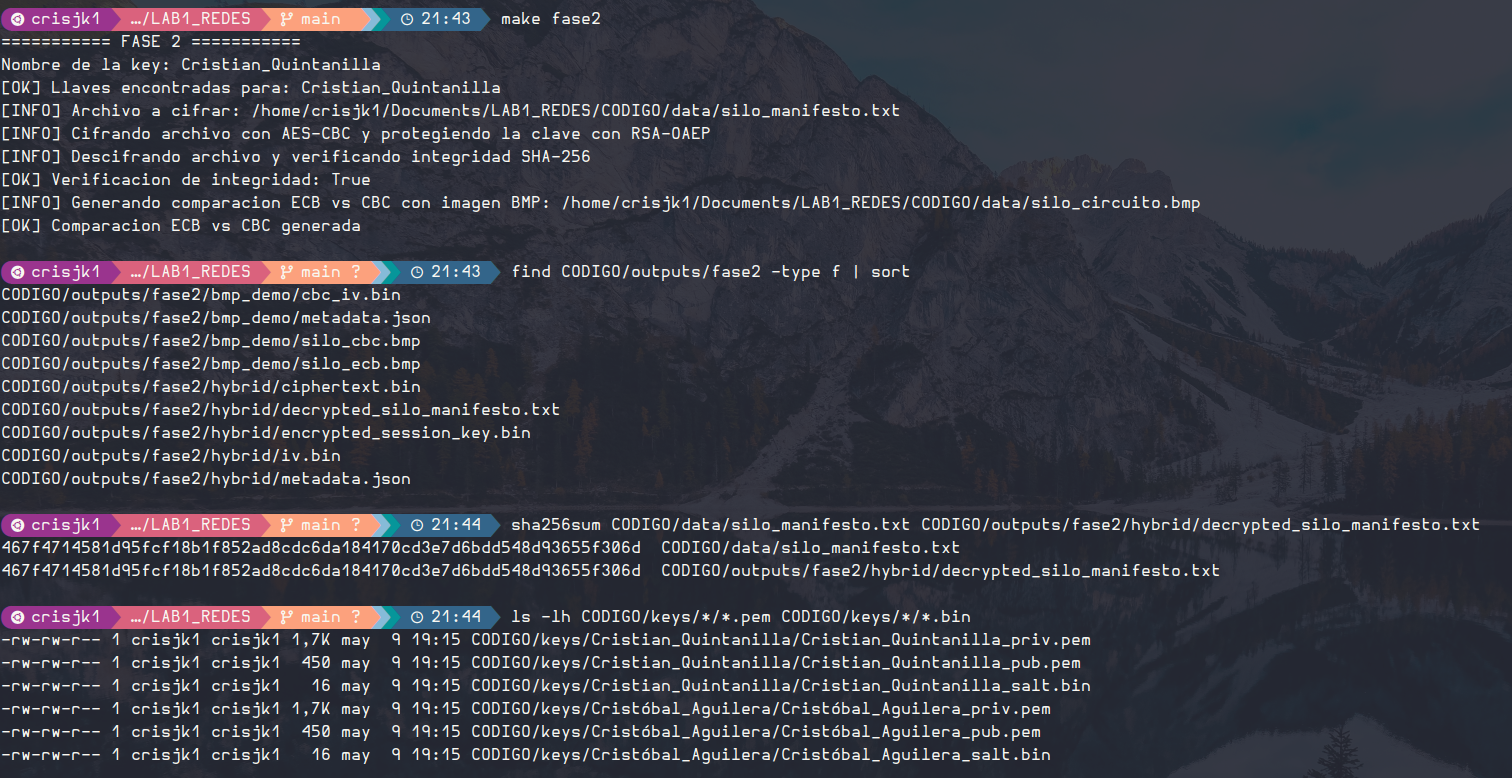
\includegraphics[width=1\textwidth]{screenshots/fase2_bash.png}
    \caption{Ejecución de Fase 2 y validación de archivos generados desde terminal.}
    \label{fig:bash_fase2}
\end{figure}

La Figura \ref{fig:comparacion_ecb_cbc} compara el resultado visual de cifrar la imagen BMP del silo en modo ECB y CBC.

\begin{figure}[H]
    \centering
    \begin{minipage}{0.48\textwidth}
        \centering
        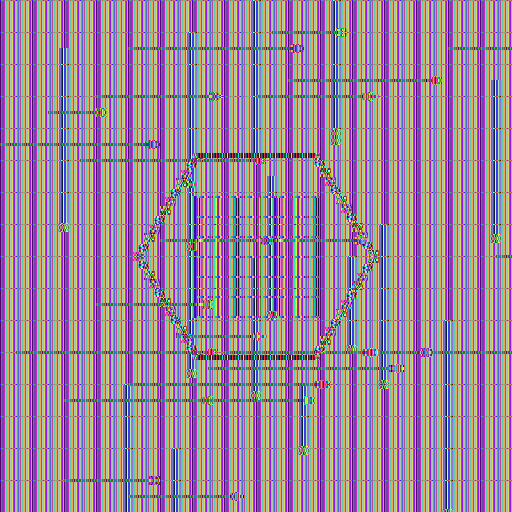
\includegraphics[width=\textwidth]{screenshots/silo_ecb.png}
        \textbf{AES-ECB}
    \end{minipage}
    \hfill
    \begin{minipage}{0.48\textwidth}
        \centering
        
\includegraphics[width=\textwidth]{screenshots/silo_cbc.png}
        \textbf{AES-CBC}
    \end{minipage}
    \caption{Comparación visual entre cifrado ECB y CBC sobre la imagen BMP del silo.}
    \label{fig:comparacion_ecb_cbc}
\end{figure}

\subsection{Análisis Teórico}
\subsubsection{Comparación ECB vs CBC}

En la fase II se cifró la imagen BMP del silo utilizando AES-128 en dos modos de operación: ECB y CBC. La diferencia observada fue clara: en la imagen cifrada con ECB todavía se distinguen patrones de la imagen original, especialmente el hexágono central, el cual se mantuvo reconocible incluso al repetir pruebas con distintas claves. Esto ocurre porque ECB cifra cada bloque de forma independiente; por lo tanto, bloques de texto plano iguales producen bloques cifrados iguales, preservando patrones estructurales en archivos con información repetitiva, como una imagen.

En cambio, al cifrar la misma imagen con CBC, los patrones visuales desaparecen completamente y el resultado se observa como ruido o estática. Esto se debe a que CBC encadena cada bloque con el bloque cifrado anterior y utiliza un IV para aleatorizar el primer bloque. Así, aunque existan bloques similares o repetidos en la imagen original, su representación cifrada cambia según el contexto del encadenamiento. Por esta razón, CBC es la mejor opción para ocultar información visual, ya que evita la filtración de patrones que sí aparece en ECB.

\section{Fase 3}

\subsection{Análisis Teórico}
En la fase III, se debe asegurar autenticidad y el no repudio de las comunicaciones del Consejo,
junto con la condicion de que no se debe saber a quien se le esta enviando el mensaje y poder comprobar la integridad de este.
Para esto hay 3 componentes principales:
\begin{itemize}
	\item \textbf{Un Hash para la integridad}: Hay que calcular un hash del mensaje original para poder verificar su integridad en la llegada.
	\item \textbf{Claves Asimetricas para autenticidad}: Hay que utilizar claves asimetricas para poder "firmar" el mensaje y asi poder confirmar la identidad de quien envia el mensaje.
	\item \textbf{Clave Simetrica compartida}: Una clave simetrica compartida permitira cifrar el mensaje sin agregar identidad al mismo, y asi cumplir la condicion de no saber a quien se le esta enviando el mensaje.
\end{itemize}

Ahora se pueden tomar 2 caminos dependiendo del orden de encriptacion, entonces el orden sera:
\begin{enumerate}
	\item \textbf{Hash}: Se calcula el hash del mensaje
	\item \textbf{Firmar}: Se firma el hash del mensaje
	\item \textbf{Encriptar}: Se encripta el mensaje junto al hash firmado
\end{enumerate}
Gracias a este orden se puede proteger la identidad de quien lo envia, ya que la firma queda bajo la proteccion de la encriptacion.
Por otro incluso si la clave simetrica compartida es comprometida, el sistema puede identificar cuales usuarios pertenecen al consejo
y denegar o alertar sobre mensajes que tengan otra identidad asociada.

\subsection{Evidencias}

En el siguiente output, se puede observar como uno de los miembros del consejo comparte la clave simetrica a un externo,
luego el externo intenta mandar mensajes al consejo:

\begin{figure}[ht]
    \centering
    \includegraphics[width=\textwidth]{screenshots/fase3-1.png}
    \caption{Evidencia de autenticidad}
    \label{fig:evidencia_fase3_1}
\end{figure}

Aun con la clave simetrica compartida, gracias a la autenticidad que proporciona la firma, es posible identificar si los mensajes
son o no enviados por miembros del consejo.
\\
\\

En este otro ouput, se puede observar como un atacante (que conoce la clave simetrica compartida) intercepta un mensaje y envia un mensaje modificado junto con la firma original:

\begin{figure}[ht]
    \centering
    \includegraphics[width=\textwidth]{screenshots/fase3-2.png}
    \caption{Evidencia de integridad}
    \label{fig:evidencia_fase3_2}
\end{figure}

Gracias a utilizar un hash bajo la firma, se puede identificar que el mensaje fue modificado y alertar sobre un sabotaje.
Especificamente en el codigo la funcion \texttt{descifrar\_mensaje} verifica la firma junto con el hash al mismo tiempo,
por lo que aun que sea un "error" de integridad igualmente el sistema intenta descifrar con las claves publicas de los
demas usuarios del consejo como si fuese un "error" de autenticidad.


\section{Fase 4}

\subsection{Evidencias}

\subsubsection{Imágenes de la simulación}

\begin{figure}[H]
    \centering
    \includegraphics[width=0.6\linewidth]{screenshots/S1.png}
    \includegraphics[width=0.2967\linewidth]{screenshots/S2.png}
    \includegraphics[width=0.2967\linewidth]{screenshots/S3.png}
\end{figure}


\subsection{Análisis Teórico}

\subsubsection{Eleccion del primo: $PRIME = 2^{521} - 1$}

Primero tenemos que escoger un numero para acotar los valores debido a que el esquema de Shamir necesita un campo  finito, este 
numero debe ser primo para que todo número no nulo sí tenga inverso multiplicativo Esto nos  garantiza que la aritmética modular 
se encuentre acotado en la cantidad de bits del secreto. Usaremos un primo de Mersenne ya que facilita todo lo anterior y es eficiente 
a nivel de software y hardware.

\begin{figure}[ht]
    \centering
    $PRIME = 2^{521} - 1$
\end{figure}

Como nuestro secreto tiene 256 bits, nuestro primo de Mersenne seleccionado es mucho mayor y garantiza que ningún secreto quede fuera 
del rango.

\subsubsection{Polinomio de grado 2}

En nuestro caso se nos pidió realizar un secreto de Shamir (3,4) por lo cual un polinomio de grado k - 1 (k = 3) garantiza que se 
necesiten 3 o mas  puntos para poder reconstruir el polinomio de Lagrange y poder acceder al secreto que se encuentra en $f(0)$. 
El caso de tener 4 llaves se genera una redundancia pero es útil en caso de que una llave se pierda.


\subsubsection{Generación del Secreto}

Para la generación de la clave secreta (secreto) utilizamos la librería secret de Python que genera aleatoriedad a través del sistema 
operativo siendo menos predecible que usar la librería random que a través de análisis complejos se puede obtener el valor. Ademas de 
que la librería encaja perfectamente con los bytes solicitados en el enunciado (32 bytes/ 256 bits) según la documentación.

\subsubsection{Reconstrucción del Secreto}

La reconstrucción se realiza mediante interpolación de Lagrange sobre el campo finito definido por el polinomio PRIME. Como el polinomio 
es de grado 2, se necesitan exactamente 3 puntos (Llaves). Evaluando el polinomio interpolado en $x = 0$ se obtiene el secreto original.

\begin{figure}[ht]
    \centering
    $f(0) = \sum_{i=0}^{k-1} y_i \cdot L_i(0)$
\end{figure}


\subsubsection{Simulacion}

En el código encontraremos una función "simulacion(f1, f2, f3, f4, secreto)" esta se encarga de simular todos los casos posibles con 1 2 3 y 4 
partes para poder acceder al secreto, este realiza interpolación de lagrange implementado en la función "interpolacion\_lagrange(puntos)" 
para luego comparar si existe un match entre el secreto original y el obtenido con la interpolación de puntos


\section{Interrogatorio}

\subsection{A) El Orden de los Factores}
\textbf{¿Por qué es vital firmar el mensaje antes de cifrarlo?} \\

Porque asi la firma queda bajo la proteccion del cifrado, de esta forma no se puede modificar la identidad asociada a la firma ni tampoco
conocer esta identidad sin saber la clave para descifrar. Si se hiciera de la forma inversa cifrando y luego firmando, alguien podria "desfirmar"
el mensaje con la clave publica del emisor y luego firmar con su propia clave privada.

\subsection{B) La Entropía de los Nombres}
\textbf{¿Cómo garantiza el SALT que no se puedan pre-calcular llaves?} \\

Sin la implementación de un SALT, la función de derivación sería puramente determinista sobre entradas predecibles (Nombre y Rol):
\begin{equation}
    Key = PBKDF2(Nombre + Rol)
\end{equation}

Esta predictibilidad permite a un atacante realizar un \textit{Ataque de Diccionario} o utilizar \textit{Rainbow Tables} (tablas de búsqueda pre-calculadas), donde se almacena una gran cantidad de combinaciones de nombres comunes y sus respectivos resultados de PBKDF2, permitiendo una recuperación de llaves casi instantánea en caso de que la base de datos sea vulnerada.

\subsection{Mecanismo de Defensa del SALT}
La inclusión de un SALT de 128 bits (16 bytes) transforma la ecuación de derivación, rompiendo la relación estática entre la identidad y la llave:
\begin{equation}
    Key = PBKDF2(Nombre + Rol + SALT)
\end{equation}

El SALT garantiza la seguridad del sistema al lograr principalmente lo siguiente:

\begin{enumerate}
    \item \textbf{Explosión del Espacio de Búsqueda:} Al introducir 128 bits de entropía adicional, el atacante ya no puede pre-calcular una tabla para un nombre. Tendría que calcular una tabla para cada una de las $2^{128}$ variaciones posibles de SALT. El almacenamiento requerido para lograr ese cálculo excede la capacidad física de los sistemas de cómputo actual.
    
    \item \textbf{Invalidez del Pre-cómputo:} El SALT obliga al atacante a realizar el esfuerzo computacional completo ($600,000$ iteraciones) de forma individual para cada miembro del equipo. No es posible reutilizar el cálculo de una identidad para otra, incluso si los nombres son idénticos, ya que cada carpeta \texttt{keys/\{nombre\}/} contiene un archivo \texttt{.bin} con un SALT único.
    
    \item \textbf{Unicidad de Salida:} Garantiza que si dos usuarios poseen el mismo nombre y rol, sus llaves RSA resultantes sean bit a bit diferentes, evitando colisiones de identidad en el repositorio compartido.
\end{enumerate}


\subsection{C) El Error del Punto Flotante}
\textbf{¿Por qué la aritmetica decimal rompe el esquema de Shamir?} \\

La interpolación de Lagrange calcula el secreto f(0) con una fórmula que involucra divisiones, multiplicaciones y sumas de números demasiado 
grandes o demasiado pequeños. Computacionalmente cada numero tiene un error de redondeo debido a los estándares (IEEE 754), cuando estos números 
se operan los errores de redondeo se se amplifican haciendo que el calculo de f(0) se impreciso y puede llevar a errores a la hora de volver a 
obtener el Secreto haciendo que el secreto original sea inservible.



\end{document}
